\documentclass[10pt,aspectratio=169]{beamer}

%\usepackage[utf8x]{inputenc}
\usepackage[T1]{fontenc}
\usepackage{lmodern}

\usepackage{amsmath,amssymb}
\usepackage{bm}
\usepackage{graphicx}
\usepackage{hyperref}
\usepackage{xcolor}

\graphicspath{{./figures/}}

\title{Bayesian analysis and naturalness of (Next-to-)Minimal SUSY Models}

\author{D.~Harries\\
  {\scriptsize
    (IPNP, Charles University in Prague)}\\
  \vspace{25pt}
  { \scriptsize
    Based on: \href{https://doi.org/10.1007/JHEP10(2017)160}{%
      P.~Athron, C.~Bal\'{a}zs, B.~Farmer, A.~Fowlie, D.~Harries,
      and D.~Kim, JHEP \textbf{10}, 160 (2017)}
    [\href{https://arxiv.org/abs/1709.07895}{arXiv:1709.07895}]
  }
}

\titlegraphic{
  \begin{center}
    \hspace*{\fill}
    
\includegraphics[scale=0.3]{uk_logo}
    \hspace*{\fill}
  \end{center}
}

\date[Phenomenology 2018, University of Pittsburgh]{May 7, 2018}

\usetheme{CambridgeUS}

\setbeamertemplate{headline}[default]{}
\setbeamertemplate{footline}[page number]{}
\setbeamertemplate{navigation symbols}{}

\begin{document}

\begin{frame}[plain]
  \titlepage
\end{frame}

\section{Naturalness Measures}

\begin{frame}
  \frametitle{Naturalness Problems}
  \begin{columns}[t]
    \begin{column}{0.5\textwidth}
      \begin{itemize} \itemsep1em
        \item Common motivation for SUSY is the hierarchy problem,
      \end{itemize}
      \begin{center}
        \includegraphics[width=0.8\textwidth]{fermionloop}
      \end{center}
      \begin{itemize} \itemsep1em
      \item Example of a \alert{``naturalness problem''}
        \begin{itemize}
        \item See also: strong CP problem, cosmological constant
          problem, flatness problem, $\ldots$
        \end{itemize}
      \end{itemize}
    \end{column}
    \begin{column}{0.5\textwidth}
      \begin{itemize} \itemsep1.5em
      \item Possible characterisation: {\color{blue} propensity of model to
        reproduce data}
      \item Related to \alert{fine-tuning}, e.g., if observations require
        a priori unjustified tuning of parameters $\Rightarrow$ model
        unnatural
      \item Prefer models in which fine-tuning not required/reduced?
      \item E.g., ``little hierarchy problem'' in MSSM
        (at tree-level)
        \begin{equation*}
          m_{h_1}^2 \leq m_Z^2 \cos^2 2\beta \, { \color{red} \lesssim
            (91 \text{ GeV})^2}
        \end{equation*}
        {\color{blue} $\Rightarrow$ non-minimal SUSY models?}
      \end{itemize}
    \end{column}
  \end{columns}
\end{frame}

\begin{frame}
  \frametitle{Quantifying Fine-tuning}
  % - claim these are problems, how do we quantify
  % - if want to use as a guide to model building/discrimination,
  %   need to be able to compare
  % - traditionally: propose measures that capture some quantity
  %   that can be mapped into naturalness
  \begin{block}{Typical Motivation}
    <model name> raises the Higgs mass at tree-level, and
    therefore is more natural than the MSSM, e.g., in the NMSSM
    \begin{equation*}
      m_{h_1}^2 \lesssim m_Z^2 \cos^2 2\beta + \frac{\lambda^2 v^2}{2}
      \sin^2 2\beta
    \end{equation*}
  \end{block}
  \begin{itemize} \itemsep1em
  \item Justify/check claim that model is more natural than another
    $\Rightarrow$ must quantify naturalness, i.e., fine-tuning
  \item \alert{But definition of fine-tuning is unclear $\ldots$}
  \end{itemize}
\end{frame}

\begin{frame}
  \frametitle{Traditional Tuning Measures}
  % - summarise relevant traditional measures and motivation of
  %   each
  % - BG measure
  % - EW measure
  % - shortcomings of traditional measures
\end{frame}

\section{Bayesian Naturalness}

\begin{frame}
  \frametitle{A Bayesian Approach}
\end{frame}

\begin{frame}
  \frametitle{Naturalness Priors}
  % - show derivation of naturalness priors
  % - introduce definition of \Delta_J
  % - summarise merits
\end{frame}

\begin{frame}
  \frametitle{Example: the SM Hierarchy Problem}
  \begin{columns}[t]
    \begin{column}{0.5\textwidth}
      \begin{figure}
        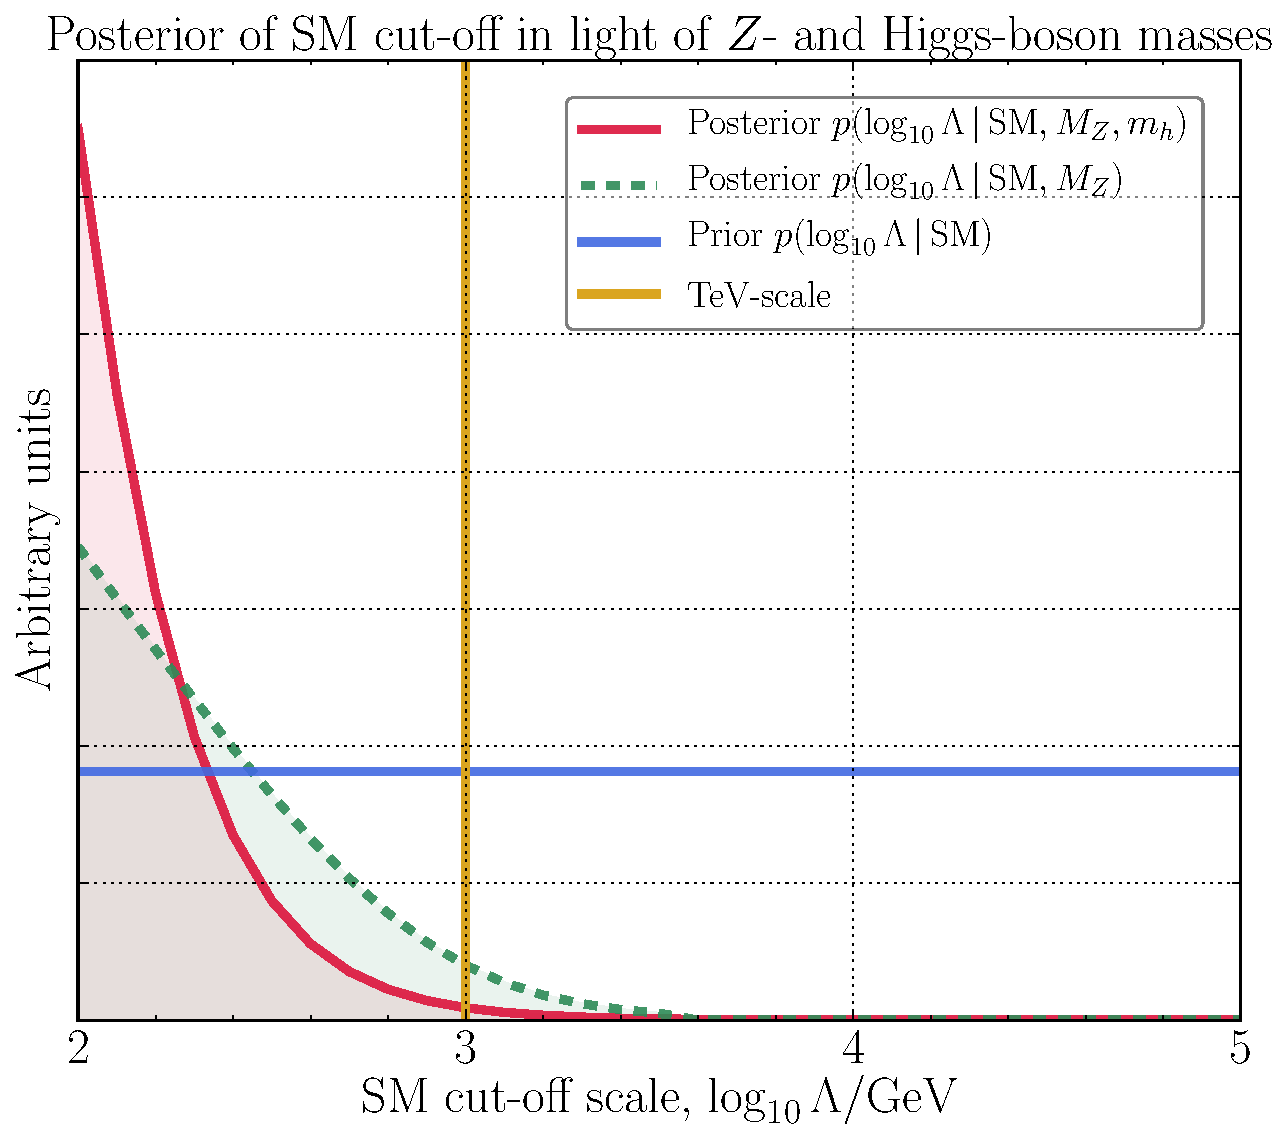
\includegraphics[width=0.9\textwidth]{SM_Lambda}
      \end{figure}
    \end{column}
    \begin{column}{0.5\textwidth}
      \begin{itemize} \itemsep1em
      \item Toy model: $M_Z^2 = -\frac{\bar{g}^2}{8 \lambda} (\mu^2
        + \Lambda_{NP}^2)$
      \item Traditional BG measure applied to, e.g., cut-off $\Lambda_{NP}^2$,
        \begin{equation*}
          \Delta_{\Lambda_{NP}^2} = \frac{\bar{g}^2}{8 \lambda}
          \frac{\Lambda_{NP}^2}{M_Z^2}
        \end{equation*}
        $\Rightarrow$ large tuning for $\Lambda_{NP}^2 \gg M_Z^2$
        \begin{itemize}
        \item But interpretation unclear, e.g., large $\Delta_{\Lambda_{NP}^2}$
          $\equiv$ implausible? When is $\Delta_{\Lambda_{NP}^2}$ too large?
        \end{itemize}
      \item Bayesian approach: posterior for $\Lambda_{NP}^2$ conditioned on
        observed $M_Z^2$, $m_h^2$
      \item Computed in terms of effective ``naturalness prior''
      \end{itemize}
    \end{column}
  \end{columns}
\end{frame}

\section{Results}

\begin{frame}
  \frametitle{Models Considered}
  % - summarise models and methods
\end{frame}

\begin{frame}
  \frametitle{Low Fine-tuning and Credible Regions}
\end{frame}

\begin{frame}
  \frametitle{Impact of $m_h \approx 125$ GeV}
\end{frame}

\begin{frame}
  \frametitle{Comparing Fine-tuning Measures}
\end{frame}

\begin{frame}
  \frametitle{Posterior Distributions}
\end{frame}

\section{Summary}

\begin{frame}
  \frametitle{Summary}
\end{frame}

\appendix

\begin{frame}
  \begin{center}
    {
      \Large
      Additional Slides
    }
  \end{center}
\end{frame}

\end{document}
